% ============================
\chapter{Un travail répétitif}
\label{chap:bcl}
% ============================

	\marginicon{objectif}
	Les ordinateurs révèlent tout leur potentiel dans leur capacité à
	répéter inlassablement les mêmes tâches.
	Vous avez pu appréhender les boucles lors de votre initiation
	sur le site \url{code.org}.
	Voyons comment utiliser à bon escient des boucles dans nos codes.

	\marginicon{attention}
	Attention~! 
	D’expérience, nous savons que ce chapitre est difficile à appréhender. 
	Beaucoup d’entre vous perdent pied ici. 
	Accrochez-vous, faites bien tous les exercices proposés,
	montrez vos solutions à votre professeur
	et demandez de l'aide dès que vous vous sentez perdu~!

% =======================================
\section{La notion de travail répétitif}
% =======================================

	Si on veut faire effectuer un travail répétitif, 
	il faut indiquer deux choses~:
	\begin{itemize}
	\item le travail à répéter ;
	\item une indication qui permet de savoir quand s'arrêter.
	\end{itemize}

	Examinons quelques exemples pour fixer notre propos.

	\paragraph{Exemple 1.} 
	Pour traiter des dossiers, 
	on dira quelque chose comme 
	«~tant qu’il reste un dossier à traiter, le traiter~» 
	ou encore 
	«~traiter un dossier puis passer au suivant jusqu’à ce qu’il n’en reste plus à traiter~».
	\begin{itemize}
	\item La tâche à répéter est : «~traiter un dossier~».
	\item On indique qu’on doit continuer s’il reste encore un dossier à traiter.
	\end{itemize}

	\paragraph{Exemple 2.}
	Pour calculer la cote finale de tous les étudiants,
	on aura quelque chose du genre 
	«~Pour tout étudiant, calculer sa cote~».
	\begin{itemize}
	\item 
		La tâche à répéter est : «~calculer la cote d’un étudiant~».
	\item 
		On indique qu’on doit le faire pour tous les étudiants.
		On doit donc commencer par le premier, passer à chaque fois au suivant
		et s’arrêter quand on a fini le dernier.
	\end{itemize}

	\paragraph{Exemple 3.}
	Pour afficher tous les nombres de 1 à 100, on aura
	«~Pour tous les nombres de 1 à 100, afficher ce nombre~».
	\begin{itemize}
	\item
		La tâche à répéter est : «~afficher un nombre~».
	\item 
		On indique qu’on doit le faire pour tous les nombres de 1 à 100. 
		On doit donc commencer avec 1, 
		passer à chaque fois au nombre suivant 
		et s’arrêter après avoir affiché le nombre 100.
	\end{itemize}
		
% ===================================================
\section{Une même instruction, des effets différents}
% ===================================================

	Comprenez bien que c’est toujours la même tâche qui est exécutée 
	mais pas avec le même effet à chaque fois. 
	Ainsi, on traite un dossier mais à chaque fois un différent ; 
	on affiche un nombre mais à chaque fois un différent. 
	
	Par exemple, la tâche à répéter pour afficher des nombres
	ne peut pas être
	\lda{\K{afficher} 1} ni \lda{\K{afficher} 2} ni\dots{}
	Par contre, on pourra utiliser l'instruction
	\lda{\K{afficher} nb} si on s'arrange pour que la variable
	\lda{nb} s'adapte à chaque passage dans la boucle.

	\begin{quote}
		\bfseries
		De façon générale,
		pour obtenir un travail répétitif,
		il faut trouver une formulation de la tâche
		qui va produire un effet différent à chaque fois.
	\end{quote}
	
	\subsection{Exemple - Afficher les nombres de 1 à 5}
	%===================================================
	
		Si on veut un algorithme qui affiche les nombres de 1 à 5
		sans utiliser de boucle, on pourrait écrire :
		
		\begin{LDA}
		\Write{1}
		\Write{2}
		\Write{3}
		\Write{4}
		\Write{5}
		\end{LDA}
		
		Ces cinq instructions sont proches mais pas tout-à-fait identiques. 
		En l'état, on ne peut pas encore en faire une boucle%
		\footnote{%
			Vous vous dites peut-être que ce code est simple ;
			inutile d'en faire une boucle.
			Ce n'est qu'un exemple.
			Que feriez-vous s'il faillait afficher les nombres
			de 1 à 1000 ?
		} ;
		il va falloir ruser.
		On peut obtenir le même résultat avec l'algorithme suivant :

		\begin{minipage}{4cm}
		\begin{LDA}
		\Let nb \Gets 1
		\Write{nb}
		\Let nb \Gets 2
		\Write{nb}
		\Let nb \Gets 3
		\Write{nb}
		\Let nb \Gets 4
		\Write{nb}
		\Let nb \Gets 5
		\Write{nb}
		\end{LDA}
		\end{minipage}
		\quad ou encore \quad
		\begin{minipage}{4cm}
		\begin{LDA}[1]
		\Let nb \Gets 1
		\Write{nb}
		\Let nb \Gets nb + 1
		\Write{nb}
		\Let nb \Gets nb + 1
		\Write{nb}
		\Let nb \Gets nb + 1
		\Write{nb}
		\Let nb \Gets nb + 1
		\Write{nb}
		\Let nb \Gets nb + 1
		\end{LDA}
		\end{minipage}
		
		Il est plus compliqué,
		mais cette fois les lignes 2 et 3 se répètent exactement.
		D'ailleurs, la dernière ligne ne sert à rien d'autre qu'à
		obtenir cinq copies identiques.
		Le travail à répéter est donc :

		\begin{LDA}
		\Write{nb}
		\Let nb \Gets nb + 1
		\end{LDA}

		Cette tâche doit être effectuée cinq fois dans notre exemple.
		Il existe plusieurs structures répétitives
		qui vont se distinguer par la façon dont on va
		contrôler le nombre de répétitions.
		Voyons-les une à une%
		\footnote{%
			Nous ne verrons pas de structure de type
			\lda{répéter 5 fois\dots}
			Elle est simple à comprendre
			mais pas souvent adaptée au problème à résoudre.
		}.

\clearpage
%========================
\section{«~tant que~»}\index{tant que}
%========================
	
	\begin{wrapfigure}{r}{6cm}
		\begin{tikzpicture}[>=triangle 60, node distance = 1.5cm, auto]
			\sffamily				
			\node[draw, diamond, aspect=2] (Test) {condition vraie ?};
			\node[draw, below of=Test] (Instr) {instructions à exécuter};
			\node[draw, circle, below of=Instr] (End) {};		          
			\draw[->] (Test) -- (Instr) node[near start] {Oui};
			\draw[->] (Test.east) to[in=0,out=0] node[near start] {Non} (End.east);
			\draw[->] (Instr.west) to[bend left] (Test.west);
		\end{tikzpicture}	
		\vspace{-1cm}
	\end{wrapfigure}
	Le «~tant que~» est une structure qui demande à
	l’exécutant de répéter une tâche (une ou plusieurs
	instructions) tant qu’une condition donnée est vraie.

	\begin{LDA}
	\While{condition}
		\Stmt séquence d’instructions à exécuter
	\EndWhile
	\end{LDA}

	Comme pour la structure \lda{si}, 
	la \lda{condition} est une expression à valeur booléenne. 
	Dans ce type de structure, 
	il faut qu’il y ait dans la séquence d’instructions comprise entre
	\lda{tant que} et \lda{fin tant que} au moins une
	instruction qui modifie une des composantes de la condition de telle
	manière qu’elle puisse devenir \textbf{fausse} à un moment donné. Dans
	le cas contraire, la condition reste indéfiniment vraie et la boucle va
	tourner sans fin, c’est ce qu’on appelle une \textbf{boucle infinie}. 
	L'ordinogramme ci-dessus décrit  le déroulement de cette structure. 
	On remarquera que si la condition est fausse dès le début, 
	la tâche n’est jamais exécutée.


	\subsection{Exemple - Afficher les nombres de 1 à 5}
	%===================================================

		Reprenons notre exemple d'affichage des nombres de 1 à 5.
		Pour rappel, la tâche à répéter est :

		\begin{LDA}
		\Write{nb}
		\Let nb \Gets nb + 1
		\end{LDA}
		
		La condition va se baser sur la valeur de \lda{nb}.
		On continue tant que le nombre n'a pas dépassé 5.
		Ce qui donne (en n'oubliant pas l'initialisation de \lda{nb}) :

		\begin{minipage}{5cm}
			\begin{LDA}[1]
				\Algo{compteur5}{}{}
					\Decl{nb}{entier}
					\Let nb \Gets 1
					\While{nb $\le$ 5}
						\Write{nb}
						\Let nb \Gets nb + 1
					\EndWhile
				\EndAlgo
			\end{LDA}
		\end{minipage}
		\quad
		\begin{minipage}{8cm}
			\begin{tabular}{|>{\centering\arraybackslash}m{6mm}
						|*{3}{>{\centering\arraybackslash}m{2cm}}|}
				\hline
					\verb_#_  & nb & condition & affichage \\			
				\hline
					2 & indéfini & {} & {} \\
					3 & 1                    & {}   & {} \\
					4 & {\color{gray}$\mid$} & vrai & {} \\
					5 & {\color{gray}$\mid$} &      & 1  \\
					6 & 2                    & {}   & {} \\
					4 & {\color{gray}$\mid$} & vrai & {} \\
					5 & {\color{gray}$\mid$} &      & 2  \\
					6 & 3                    & {}   & {} \\
					4 & {\color{gray}$\mid$} & vrai & {} \\
					5 & {\color{gray}$\mid$} &      & 3  \\
					6 & 4                    & {}   & {} \\
					4 & {\color{gray}$\mid$} & vrai & {} \\
					5 & {\color{gray}$\mid$} &      & 4  \\
					6 & 5                    & {}   & {} \\
					4 & {\color{gray}$\mid$} & vrai & {} \\
					5 & {\color{gray}$\mid$} &      & 5  \\
					6 & 6                    & {}   & {} \\
					4 & {\color{gray}$\mid$} & faux & {} \\
				\hline
			\end{tabular}
		\end{minipage}

	\subsection{Exemple - Généralisation à n nombres}
	%===================================================

		On peut généraliser l'exemple précédent
		en affichant tous les nombres de 1 à n où n est une donnée
		de l'algorithme.
		
		\begin{LDA}
		\Algo{compteur}{\Par{n}{entier}}{}
			\Decl{nb}{entier}
			\Let nb \Gets 1
			\While{nb $\le$ n}
				\Write{nb}
				\Let nb \Gets nb + 1
			\EndWhile
		\EndAlgo
		\end{LDA}

	\subsection{Exercices}
	% =====================================

		\begin{Exercice}{Compréhension d’algorithmes}
			Quels sont les affichages réalisés lors de l’exécution
			des algorithmes suivants~?
			
			\begin{minipage}[t]{40mm}
				\begin{LDA}
				\Algo{boucle1}{}{}
					\Decl{x}{entier}
					\Let x \Gets 0
					\While{x < 12}
						\Let x \Gets x + 2	
					\EndWhile
					\Write x
				\EndAlgo
				\end{LDA}
			\end{minipage}
			\ 
			\begin{minipage}[t]{45mm}
				\begin{LDA}
				\Algo{boucle2}{}{}
					\Decl{ok}{booléen}
					\Decl x : entier
					\Let ok \Gets vrai
					\Let x \Gets 5
					\While{ok}
						\Let x \Gets x + 7	
						\Let ok \Gets x MOD 11 $\neq$ 0	
					\EndWhile
					\Write x
				\EndAlgo
				\end{LDA}
			\end{minipage}
			\ 
			\begin{minipage}[t]{50mm}
				\begin{LDA}
				\Algo{boucle3}{}{}
					\Decl{ok}{booléen}
					\Decl cpt, x : entiers
					\Let x \Gets 10
					\Let cpt \Gets 0
					\Let ok \Gets vrai
					\While{ok ET cpt < 3}
						\If{x MOD 2 = 0}
							\Let x \Gets x + 1
							\Let ok \Gets x < 20
						\Else
							\Let x \Gets x + 3
							\Let cpt \Gets cpt + 1
						\EndIf
					\EndWhile
					\Write x
				\EndAlgo
				\end{LDA}
			\end{minipage}
		\end{Exercice}

		\begin{Exercice}{Afficher des nombres}
			En utilisant un \lda{\algorithmicwhile},
			écrire un algorithme qui reçoit un entier $n$ positif et affiche
			\begin{enumerate}[label=\alph*)]
			\item les nombres de 1 à $n$ ;
			\item les nombres de 1 à $n$ en ordre décroissant ;
			\item les nombres impairs de 1 à $n$ ;
			\item les nombres de -n à n ;
			\item les multiples de 5 de 1 à n ;
			\item les multiples de n de 1 à 100.
			\end{enumerate}
		\end{Exercice}

\clearpage
%====================
\section{«~pour~»}\index{pour}
%====================

	\begin{wrapfigure}{r}{7cm}
		\begin{tikzpicture}[>=triangle 60, node distance = 1.5cm, auto]
			\sffamily				
			\node[draw] (Init) {variable \Gets début};
			\node[draw, diamond, aspect=2, below of=Init] (Test) {variable $\leq$ fin ?};
			\node[draw, below of=Test] (Instr) {instructions à exécuter};
			\node[draw, below of=Instr] (Incr) {variable \Gets variable + pas};
			\node[draw, circle, below of=Incr] (End) {};		          
			\draw[->] (Init) -- (Test);
			\draw[->] (Test) -- (Instr) node[near start] {Vrai};
			\draw[->] (Test.east) to[in=-30,out=0] node[near start] {Faux} (End.south);
			\draw[->] (Instr) -- (Incr);
			\draw[->] (Incr.west) to[bend left] (Test.west);
		\end{tikzpicture}	
		\vspace{-2cm}
	\end{wrapfigure}

	Ici, on va plutôt indiquer 
	\textbf{combien de fois} la tâche doit être répétée. 
	Cela se fait au travers d’une
	\textbf{variable de contrôle} dont la valeur va évoluer à partir
	d’une valeur de départ jusqu’à une valeur finale.
	
	\begin{LDA}
	\For[pas]{variable}{début}{fin}
		\Stmt séquence d’instructions à exécuter
	\EndFor
	\end{LDA}

	Dans ce type de structure, 
	\lda{début}, \lda{fin} et \lda{pas}
	peuvent être des constantes, 
	des variables ou des expressions entières. 

	Le \lda{pas} est facultatif, et généralement omis 
	(dans ce cas, sa valeur par défaut est 1). 

	La boucle s’arrête
	lorsque la variable dépasse la valeur de \lda{fin}. 

	La variable de contrôle ne servant que pour la boucle
	et étant forcement entière,
	on va considérer qu'il n'est pas nécessaire de la déclarer
	et qu'elle n'est pas utilisable en dehors de la boucle%
	\footnote{%
		De nombreux langages ne le permettent d'ailleurs pas
		ou ont un comportement indéterminé si on le fait.%
	}.

	\subsection{Exemples}
	%===================================================

		Reprenons notre exemple d'affichage des nombres de 1 à 5.
		Voici la solution avec un \lda{\algorithmicfor} 
		et le traçage corrrespondant.

		\begin{minipage}{55mm}
			\begin{LDA}[1]
				\Algo{compterJusque5}{}{}
					\LComment par défaut le pas est de 1
					\For{nb}{1}{5} 
						\Write nb 
					\EndFor
				\EndAlgo
			\end{LDA}
		\end{minipage}
		\qquad
		\begin{minipage}{75mm}
			\begin{tabular}{|>{\centering\arraybackslash}m{6mm}
						|*{3}{>{\centering\arraybackslash}m{15mm}}|}
				\hline
					\verb_#_  & nb & condition & affichage \\			
				\hline
					3 & 1                    & vrai & {} \\
					4 & {\color{gray}$\mid$} &      & 1  \\
					3 & 2                    & vrai & {} \\
					4 & {\color{gray}$\mid$} &      & 2  \\
					3 & 3                    & vrai & {} \\
					4 & {\color{gray}$\mid$} &      & 3  \\
					3 & 4                    & vrai & {} \\
					4 & {\color{gray}$\mid$} &      & 4  \\
					3 & 5                    & vrai & {} \\
					4 & {\color{gray}$\mid$} &      & 5  \\
					3 & 6                    & faux & {} \\
				\hline
			\end{tabular}
		\end{minipage}

		Si on veut généraliser l'affichage à n nombres, on a :
		
		\begin{LDA}
		\Algo{compterJusqueN}{\Par{n}{entier}}{}
			\For{nb}{1}{n}
				\Write nb 
			\EndFor
		\EndAlgo
		\end{LDA}

\clearpage
	\subsection{Un pas négatif}
	%===================================================

		\begin{wrapfigure}{r}{6cm}
			\begin{tikzpicture}[>=triangle 60, node distance = 1.5cm, auto]
				\sffamily				
				\node[draw] (Init) {variable \Gets début};
				\node[draw, diamond, aspect=2, below of=Init] (Test) {variable $\geq$ fin ?};
				\node[draw, below of=Test] (Instr) {instructions à exécuter};
				\node[draw, below of=Instr] (Incr) {variable \Gets variable + pas};
				\node[draw, circle, below of=Incr] (End) {};		          
				\draw[->] (Init) -- (Test);
				\draw[->] (Test) -- (Instr) node[near start] {Vrai};
				\draw[->] (Test.east) to[in=-30,out=0] node[near start] {Faux} (End.south);
				\draw[->] (Instr) -- (Incr);
				\draw[->] (Incr.west) to[bend left] (Test.west);
			\end{tikzpicture}	
			\vspace{-3cm}
		\end{wrapfigure}

		Le pas est parfois négatif, dans le cas d’un compte à rebours, 
		par exemple.
		Dans ce cas, 
		la boucle s’arrête
		lorsque la variable prend une valeur 
		plus petite que la valeur de \lda{fin}
		(cf. le test dans l’organigramme ci-contre).

		\textbf{Exemple} : Compte à rebours à partir de n.
		
		\begin{LDA}
		\Algo{compterÀReboursDécroissant}{\Par{n}{entier}}{}
			\For[-1]{nb}{n}{1}
				\Write nb 
			\EndFor
			\Write "Partez !"
		\EndAlgo
		\end{LDA}

	\subsection{Cohérence}
	%===================================================

		Il faut veiller à la cohérence de l’écriture de cette structure. On considérera
		qu’au cas (à éviter) où \lda{début} est strictement supérieur à
		\lda{fin} et le \lda{pas} est positif, la séquence d’instructions
		n’est jamais exécutée (mais ce n’est pas le cas dans tous les langages
		de programmation~!). Idem si \lda{début} est strictement inférieur à
		\lda{fin} mais avec un \lda{pas} négatif.
	
		\textbf{Exemples~}:
	
		\begin{LDA}
		\Stmt \K{pour} i \K{de} 2 \K{à} 0 \K{faire} \RComment La boucle n’est pas exécutée.
		\Stmt \K{pour} i \K{de} 1 \K{à} 10 \K{par} -1 \K{faire} \RComment La boucle n’est pas exécutée.
		\Stmt \K{pour} i \K{de} 1 \K{à} 1 \K{par} 5 \K{faire} \RComment La boucle est exécutée 1 fois.
		\end{LDA}

	\subsection{Modification des variables de contrôle}
	%===================================================
		
		\marginicon{attention}
		Il est important de ne pas modifier 
		dans la séquence d’instructions une des
		variables de contrôle \lda{début}, \lda{fin} ou \lda{pas}~! 
		Il est aussi fortement déconseillé de modifier «~manuellement~» la
		\lda{variable} de contrôle au sein de la boucle
		\lda{pour}. 
		Il ne faut pas l’initialiser en début de boucle,
		et ne pas s’occuper de sa modification, l’instruction 
		\lda{i \Gets i + pas} 
		étant automatique et implicite à chaque étape de la boucle. 
	
	\subsection{Exemple -- Afficher uniquement les nombres pairs}
	%===========================================================

		Cette fois-ci on affiche uniquement 
		les nombres \textbf{pairs} jusqu’à la limite $n$.
		
		\textbf{Exemple :}
		Les nombres pairs de $1$ à $10$ sont~: $2$, $4$, $6$, $8$, $10$.
		
		Notez que $n$ peut être impair. 
		Si $n$ vaut $11$, l’affichage est le même que pour $10$.
		On peut utiliser un \og{}pour\fg{}.
		Une solution possible est :

		\begin{LDA}
		\Algo{afficherPair}{\Par{n}{entier}}{} 
			\For[2]{nb}{2}{n} 
				\Write nb 
			\EndFor
		\EndAlgo
		\end{LDA}

		La section sur les suites proposera d'autres solutions
		pour ce problème.
		
	\subsection{Exercices}
	% =====================================

		\begin{Exercice}{Compréhension d’algorithmes}
			Quels sont les affichages réalisés lors de l’exécution
			des algorithmes suivants~?
			
			\begin{minipage}[t]{6cm}
				\begin{LDA}
				\Algo{boucle5}{}{}
					\Decl{x}{entier}
					\Decl{ok}{booléen}
					\Let x \Gets 3
					\Let ok \Gets vrai
					\For{i}{1}{5}
						\Let x \Gets x + i
						\Let ok \Gets ok ET (x MOD 2 = 0)
					\EndFor
					\If{ok}
						\Write x
					\Else
						\Write 2 * x
					\EndIf
				\EndAlgo
				\end{LDA}
			\end{minipage}
			\quad
			\begin{minipage}[t]{6cm}
				\begin{LDA}
				\Algo{boucle6}{}{}
					\Decl{fin}{entiers}
					\For{i}{1}{3}
						\Let fin \Gets 6 * i - 11
						\For[3]{j}{1}{fin}
							\Write 10 * i + j
						\EndFor
					\EndFor
				\EndAlgo
				\end{LDA}
			\end{minipage}

		\end{Exercice}

		\begin{Exercice}{Afficher des nombres}
			Reprenons un exercice déjà donné avec le \lda{\algorithmicwhile}.
			En utilisant un \lda{\algorithmicfor},
			écrire un algorithme qui reçoit un entier $n$ positif et affiche
			\begin{enumerate}[label=\alph*)]
			\item les nombres de 1 à $n$ ;
			\item les nombres de 1 à $n$ en ordre décroissant ;
			\item les nombres de -n à n ;
			\item les multiples de 5 de 1 à n ;
			\item les multiples de n de 1 à 100.
			\end{enumerate}
		\end{Exercice}

%===================================
\section{«~faire~–~tant que~»}
%===================================

	\begin{wrapfigure}{r}{4cm}
		\begin{tikzpicture}[>=triangle 60, node distance = 2cm, auto]
			\sffamily
			\node[draw] (Instr) {instructions à exécuter};
			\node[draw, diamond, aspect=2, below of=Instr] (Test) {Condition vraie ?};
			\node[draw, circle, below of=Test] (End) {};		          
			\draw[->] (Instr) -- (Test);
			\draw[->] (Test) -- (End) node[near start] {Non};
			\draw[->] (Test.east) to[in=0,out=0] node[near start] {Oui} (Instr.east);
		\end{tikzpicture}	
	\end{wrapfigure}

	Cette structure est très proche du «faire~-~tant que~» 
	à ceci près que le test est fait à la fin et pas au début%
	\footnote{%
		Certains langages introduisent aussi (ou à la place)
		un \lda{K{faire jusqu'à ce que}}.
		Dans ce cas, la boucle continue lorsque le test est
		\textbf{faux} et s'arrête lorsqu'il est vrai.
	}. 
	La tâche est donc toujours exécutée au moins une fois.

	\begin{LDA}
	\Repeat
		\Stmt séquence d’instructions à exécuter
	\EndRepeat{condition}
	\end{LDA}

	Comme avec le tant-que, 
	il faut que la séquence d’instructions comprise entre
	\lda{\K{faire}} et \lda{\K{tant que}} 
	contienne au moins une instruction qui modifie la condition de
	telle manière qu’elle puisse devenir \textbf{vraie} à un moment donné
	pour arrêter l’itération. 
	Le schéma ci-contre décrit le déroulement de cette boucle. 

	\subsection{Exemple}
	%===================================================

		Reprenons notre exemple d'affichage des nombres de 1 à 5.
		Voici la solution et le traçage corrrespondant.

		\begin{minipage}{5cm}
			\begin{LDA}[1]
				\Algo{compteur5}{}{}
					\Decl{nb}{entier}
					\Let nb \Gets 1
					\Repeat
						\Write{nb}
						\Let nb \Gets nb + 1
					\EndRepeat{nb $\le$ 5}
				\EndAlgo
			\end{LDA}
		\end{minipage}
		\quad
		\begin{minipage}{8cm}
			\begin{tabular}{|>{\centering\arraybackslash}m{6mm}
						|*{3}{>{\centering\arraybackslash}m{2cm}}|}
				\hline
					\verb_#_  & nb & condition & affichage \\			
				\hline
					2 & indéfini & {} & {} \\
					3 & 1                    & {}   & {} \\
					5 & {\color{gray}$\mid$} &      & 1  \\
					6 & 2                    & {}   & {} \\
					7 & {\color{gray}$\mid$} & vrai & {} \\
					5 & {\color{gray}$\mid$} &      & 2  \\
					6 & 3                    & {}   & {} \\
					7 & {\color{gray}$\mid$} & vrai & {} \\
					5 & {\color{gray}$\mid$} &      & 3  \\
					6 & 4                    & {}   & {} \\
					7 & {\color{gray}$\mid$} & vrai & {} \\
					5 & {\color{gray}$\mid$} &      & 4  \\
					6 & 5                    & {}   & {} \\
					7 & {\color{gray}$\mid$} & vrai & {} \\
					5 & {\color{gray}$\mid$} &      & 5  \\
					6 & 6                    & {}   & {} \\
					7 & {\color{gray}$\mid$} & faux & {} \\
				\hline
			\end{tabular}
		\end{minipage}

	\subsection{Exercices}
	%===================================================
	
		\begin{Exercice}{Compréhension d’algorithmes}
			Quels sont les affichages réalisés lors de l’exécution
			des algorithmes suivants~?

			\begin{LDA}
				\Algo{boucle4}{}{}
					\Decl{pair, grand}{booléens}
					\Decl{p, x}{entiers}
					\Let x \Gets 1
					\Let p \Gets 1
					\Repeat
						\Let p \Gets 2 * p
						\Let x \Gets x + p
						\Let pair \Gets x MOD 2 = 0
						\Let grand \Gets x > 15
					\EndRepeat{NON pair ET NON grand}
					\Write x
				\EndAlgo
			\end{LDA}			
		
		\end{Exercice}

		\begin{Exercice}{Afficher des nombres}
			Reprenons un exercice déjà fait avec le \lda{\algorithmicwhile}
			et le \lda{\algorithmicfor}
			en utilisant cette fois un \lda{\algorithmicuntil}.
			Écrire un algorithme qui reçoit un entier $n$ positif et affiche
			\begin{enumerate}[label=\alph*)]
			\item les nombres de 1 à $n$ ;
			\item les nombres de 1 à $n$ en ordre décroissant ;
			\item les nombres de -n à n ;
			\item les multiples de 5 de 1 à n ;
			\item les multiples de n de 1 à 100.
			\end{enumerate}
		\end{Exercice}

%======================================
\section{Quel type de boucle choisir~?}
%======================================

	En pratique, il est possible d’utiliser systématiquement la boucle 
	\lda{tant que} qui peut s’adapter à toutes les situations. 
	Cependant, il est plus clair d’utiliser la boucle \lda{pour} 
	dans les cas où le nombre d’itérations est fixé et connu à l’avance 
	(par là, on veut dire que le nombre d’itérations est déterminé au moment 
	où on arrive à la boucle). 
	La boucle \lda{faire} convient quant à elle
	dans les cas où le contenu de la boucle doit être parcouru au moins une
	fois, alors que dans \lda{tant que}, 
	le nombre de parcours peut être nul si la condition initiale est fausse. 
	La schéma ci-dessous propose un récapitulatif.

	\begin{center}
		\bigskip
		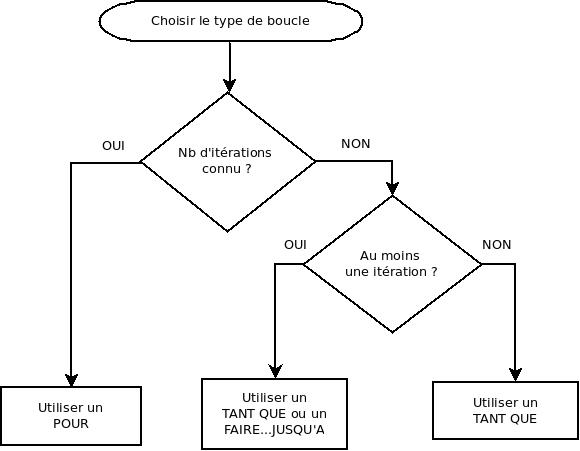
\includegraphics[width=.8\textwidth]{image/boucle-choixtype}
				\label{fig:boucle-choix}
	\end{center}

	
% ================================
\section{Acquisition de données multiples}
% ================================

	Il existe des problèmes
	où l'algorithme doit demander une série de valeurs
	à l'utilisateur pour pouvoir les traiter.
	Par exemple, les sommer, en faire la moyenne,
	calculer la plus grande\dots
	
	Dans ce genre de problème,
	on va devoir stocker chaque valeur donnée par l'utilisateur 
	dans une seule et même variable et la traiter avant de passer
	à la suivante.
	Prenons un exemple concret pour mieux comprendre.

	\begin{quote}
	On veut pouvoir calculer (et retourner)
	la somme d’une série de nombres donnés par l’utilisateur. 
	\end{quote}

	Il faut d’abord se demander 
	comment l’utilisateur va pouvoir indiquer
	combien de nombres il faut additionner 
	ou quand est-ce que le dernier nombre à additionner a été entré. 
	Voyons quelques possibilités.
	
	\clearpage
	\subsection{Variante 1 : nombre de valeurs connu} 
	%------------------------------------------------	
	
		L’utilisateur indique le nombre de termes au départ.
		Ce problème est proche de ce qui a déjà été fait.
		
		\begin{LDA}
		\LComment Lit des valeurs entières et retourne la somme des valeurs lues.
		\Algo{sommeNombres}{}{entier} \RComment Variante 1
			\Decl{nbValeurs}{entier} \RComment nb de valeurs à additionner
			\Decl{valeur}{entier} \RComment un des termes de l’addition
			\Decl{somme}{entier} \RComment la somme
			\Let somme \Gets 0 \RComment la somme se construit petit à petit. 0 au départ
			\Read nbValeurs
			\For{i}{1}{nbValeurs}
				\Read valeur
				\Let somme \Gets somme + valeur 
			\EndFor
			\Return somme
		\EndAlgo
		\end{LDA}

		\begin{Exercice}{Afficher les nombres impairs}
			Écrire un algorithme qui demande une série
			de valeurs entières à l'utilisateur
			et qui affiche celles qui sont impaires.
			L'algorithme commence par demander à l'utilisateur
			le nombre de valeurs qu'il désire donner.
		\end{Exercice}
			
	\subsection{Variante 2 : stop ou encore}
	%------------------------------------------------	
	
		Après chaque nombre, 
		on demande à l’utilisateur s’il y a encore un nombre à additionner.

		Ici, il faut chercher une solution différente
		car on ne connait pas au départ le nombre de valeurs à additionner et
		donc le nombre d’exécution de la boucle. On va devoir passer à un
		«~tant que~» ou un «faire - jusqu’à ce que». On peut
		envisager de demander en fin de boucle s’il reste
		encore un nombre à additionner. Ce qui donne~:

		\begin{LDA}
		\LComment Lit des valeurs entières et retourne la somme des valeurs lues.
		\Algo{sommeNombres}{}{entier} \RComment Variante 2a
			\Decl{encore}{booléen} \RComment est-ce qu’il reste encore une valeur à additionner~?
			\Decl{valeur}{entier} \RComment un des termes de l’addition
			\Decl{somme}{entier} \RComment la somme
			\Let somme \Gets 0
			\Repeat 
				\Read valeur
				\Let somme \Gets somme + valeur 
				\Read encore
			\EndRepeat{NON encore}
			\Return somme
		\EndAlgo
		\end{LDA}
		
		Avec cette solution, on additionne au moins une valeur. 
		Si on veut pouvoir tenir compte du
		cas très particulier où l’utilisateur ne veut
		additionner aucune valeur, il faut utiliser un «~tant que~» et donc
		poser la question avant d’entrer dans la boucle.

		\begin{LDA}
		\LComment Lit des valeurs entières et retourne la somme des valeurs lues.
		\Algo{sommeNombres}{}{entier} \RComment Variante 2b
			\Decl{encore}{booléen} \RComment est-ce qu’il reste encore une valeur à additionner~?
			\Decl{valeur}{entier} \RComment un des termes de l’addition
			\Decl{somme}{entier} \RComment la somme
			\Let somme \Gets 0
			\Read encore
			\While{encore} 
				\Read valeur
				\Let somme \Gets somme + valeur 
				\Read encore
			\EndWhile
			\Return somme
		\EndAlgo
		\end{LDA}

		\begin{Exercice}{Compter les nombres impairs}
			Écrire un algorithme qui demande une série
			de valeurs entières à l'utilisateur
			et qui lui affiche le nombre de valeurs impairs
			qu'il a donné.
			Après chaque valeur entrée,
			l'algorithme demande à l'utilisateur s'il y en a encore d'autres.
		\end{Exercice}

	\subsection{Variante 3 : valeur sentinelle}
		
		L’utilisateur entre une valeur spéciale pour indiquer la fin. 
		On parle de valeur \textbf{sentinelle}. 
		Ceci n’est possible que si cette valeur \textbf{sentinelle} ne peut pas être
		un terme valide de l’addition. Par exemple, si on veut
		additionner des nombres positifs uniquement, la valeur -1 peut servir
		de valeur sentinelle. Mais sans limite sur les nombres à additionner
		(positifs, négatifs ou nuls) il n’est pas possible de
		choisir une sentinelle.

		Ici, on se base sur la valeur entrée pour décider si on continue ou pas. 
		Il faut donc \textbf{toujours} effectuer un test
		après une lecture de valeur. C’est pour cela
		qu’il faut effectuer une lecture avant et une autre à
		la fin de la boucle.

		\begin{LDA}
		\LComment Lit des valeurs entières et retourne la somme des valeurs lues.
		\Algo{sommeNombres}{}{entier} \RComment Variante 3
			\Decl{valeur}{entier} \RComment un des termes de l’addition
			\Decl{somme}{entier} \RComment la somme
			\Let somme \Gets 0
			\Read valeur
			\While{valeur ${\geq}$ 0} 
				\Let somme \Gets somme + valeur 
				\Read valeur \RComment remarquer l’endroit où on lit une valeur.
			\EndWhile
			\Return somme
		\EndAlgo
		\end{LDA}

		\begin{Exercice}{Choix de la valeur sentinelle}
			Quelle valeur sentinelle prendrait-on 
			pour additionner une série de cotes d’interrogations~? 
			Une série de températures~?
		\end{Exercice}

		\begin{Exercice}{Afficher les nombres impairs}
			Écrire un algorithme qui demande une série
			de valeurs entières non nulles à l'utilisateur
			et qui affiche celles qui sont impaires
			La fin des données sera signalée 
			par la valeur sentinelle 0.
		\end{Exercice}

		\begin{Exercice}{Compter le nombre de réussites}
			Écrire un algorithme qui demande une série
			de cotes (entières, sur 20) à l'utilisateur
			et qui affiche le pourcentage de réussites.
			La fin des données sera signalée 
			par une valeur sentinelle que vous pouvez choisir.
		\end{Exercice}


% ================================
\section{Les suites}
% ================================

	Nous avons vu quelques exemples d'algorithmes
	qui affichent une suite de nombres
	(par exemple, afficher les nombres pairs).
	Nous avons pu les résoudre facilement
	avec un \lda{\algorithmicfor}
	en choisissant judicieusement les valeurs de début et de fin
	ainsi que le pas.
	
	Ce n'est pas toujours aussi simple.
	Nous allons voir deux exemples plus complexes
	et les solutions qui vont avec.
	Elles pourront se généraliser à beaucoup d'autres exemples.
	
	\subsubsection{Exemple - Afficher les carrés}
	%--------------------------------------------
	
		On veut afficher les $n$ premiers nombres carrés parfaits :
		$1$, $4$, $9$, $16$, $25$\dots

		Si on vous demande : "Quel est le 7\ieme{} nombre à afficher ?".
		Vous répondrez : "Facile ! C'est $7^2$, soit $49$".
		Plus généralement, le nombre à afficher 
		lors du $i$\ieme{} passage dans la boucle est $i^2$.

		\begin{tabular}{l|*{8}{>{\centering\arraybackslash}m{8mm}}}
		 étape & 1 & 2 & 3 & 4 & 5 & 6 & 7 & 8\\\hline
		 valeur à afficher & 1 & 4 & 9 & 16 & 25 & 36 & 49 & 64 \\
		\end{tabular}
		
		L'algorithme qui en découle est :
		
		\begin{LDA}
			\Algo{suiteCarrés}{\Par{n}{entier}}{}
				\For{i}{1}{n}
					\Write $i^2$
				\EndFor
			\EndAlgo
		\end{LDA}

		Dans cette solution,
		la variable de contrôle compte simplement le nombre d’itérations.
		On calcule le nombre à afficher en fonction cette variable de contrôle 
		(ici le carré convient).
		Par une vieille habitude des programmeurs%
		\footnote{%
			Née avec le langage FORTRAN 
			où la variable $i$ était par défaut une variable entière.
		},
		une variable de contrôle 
		qui se contente de compter les passages dans la boucle 
		est souvent nommée $i$. 
		On l’appelle aussi «~itérateur~».	

		Cette solution peut être utilisée
		chaque fois qu'on peut calculer le nombre à afficher
		en fonction de $i$.
		
	\subsubsection{Exemple - Une suite un peu plus complexe}
	%-------------------------------------------------------
	 
		Écrire un algorithme qui affiche 
		les $n$ premiers nombres de la suite :
		1, 2, 4, 7, 11, 16\dots{}
		
		Comme on peut le constater, 
		à chaque étape on ajoute un peu plus au nombre précédent.
		\[ 
			1 
			\xrightarrow{+1} 2 
			\xrightarrow{+2} 4
			\xrightarrow{+3} 7 
			\xrightarrow{+4} 11 
			\xrightarrow{+5} 16 
			\dots
		\] 

		Ici, difficile de partir de la solution de l'exemple précédent
		car il est n'est pas facile de trouver la fonction $f(i)$
		qui permet de calculer le nombre à afficher en fonction de i. 
		
		Par contre, il est assez simple de calculer ce nombre 
		en fonction du précédent.
		\[
			\mbox{nb à afficher} = \mbox{nb affiché juste avant} + i
		\]
		Sauf pour le premier, qui ne peut pas être calculé
		en fonction du précédent.
		Une solution élégante et facilement adaptable
		à d'autres situations est :
		
		\begin{LDA}
			\Algo{suite}{\Par{n}{entier}}{}
				\Decl{val}{entier}
				\Let val \Gets \textit{1\iere{} valeur à afficher}
				\For{i}{1}{n}
					\Write val
					\Let val \Gets \textit{la valeur suivante calculée à partir de la valeur courante}
				\EndFor
			\EndAlgo
		\end{LDA}
		
		qui, dans notre exemple précis, devient :

		\begin{LDA}
			\Algo{suite}{\Par{n}{entier}}{}
				\Decl{val}{entier}
				\Let val \Gets 1
				\For{i}{1}{n}
					\Write val
					\Let val \Gets val + i
				\EndFor
			\EndAlgo
		\end{LDA}

	\subsubsection{Exercices}
	%-------------------------------------------------------
		
		\begin{Exercice}{Suites}
			Écrire les algorithmes qui affichent
			les $n$ premiers termes des suites suivantes.
			À vous de voir quel est le canevas de solution
			le plus adapté.
			\begin{enumerate}[label=\alph*)]
			\item -1, -2, -3, -4, -5, -6\dots
			\item 1, 3, 6, 10, 15, 21, 28\dots
			\item 1, 0, 1, 0, 1, 0, 1, 0\dots
			\item 1, 2, 0, 1, 2, 0, 1, 2\dots
			\item 1, 2, 3, 1, 2, 3, 1, 2\dots
			\item 1, 2, 3, 2, 1, 2, 3, 2\dots
			\end{enumerate}			
		\end{Exercice}
				
% ================================
\section{Exercices récapitulatifs}
% ================================

	\begin{Exercice}{Factorielle}
		Écrire un algorithme qui retourne la factorielle de $n$ (entier positif ou
		nul). Rappel~: la factorielle de $n$, notée $n$!, est le produit des $n$
		premiers entiers strictement positifs. 
		
		Par convention, 0! = 1.
	\end{Exercice}
	
	\begin{Exercice}{Produit de 2 nombres}
		Écrire un algorithme qui retourne le produit de deux entiers quelconques
		sans utiliser l’opérateur de multiplication, mais en minimisant le
		nombre d’opérations.
	\end{Exercice}
	
	\begin{Exercice}{Nombre premier}
		Écrire un algorithme qui vérifie si un entier positif est un
		\textbf{nombre premier}. 
		
		Rappel~:~un nombre est premier s’il n’est divisible que par 1 et par
		lui-même. Le premier nombre premier est 2.
	\end{Exercice}
	
	\begin{Exercice}{Nombres premiers}
		Écrire un algorithme qui affiche les nombres premiers inférieurs ou
		égaux à un entier positif donné. Le module de cet algorithme fera appel
		de manière répétée mais économique à celui de l’exercice précédent.
	\end{Exercice}

	\begin{Exercice}{Somme de chiffres}
		\marginicon{java}
		Écrire un algorithme qui calcule la somme des chiffres qui forment un
		nombre naturel $n$. Attention, on donne au départ \textbf{le} nombre et
		pas ses chiffres. Exemple~: 133045 doit donner comme résultat 16,
		car 1 + 3 + 3 + 0 + 4 + 5 = 16.
	\end{Exercice}
	
	\begin{Exercice}{Nombre parfait}
		Écrire un algorithme qui vérifie si un entier positif est un
		\textbf{nombre parfait}, c’est-à-dire un nombre égal à la somme de ses
		diviseurs (sauf lui-même). 
		
		Par exemple, 6 est parfait car 6 = 1 + 2 + 3. 
		De même, 28 est parfait car 28 = 1 + 2 + 4 + 7 + 14.
	\end{Exercice}
	
	\begin{Exercice}{Décomposition en facteurs premiers}
		Écrire un algorithme qui affiche la décomposition 
		d’un entier en facteurs premiers. 
		Par exemple, $1001880$ donnerait comme décomposition
		$2^3 * 3^2 * 5 * 11^2 * 23$.
	\end{Exercice}

	\begin{Exercice}{Nombre miroir}
		Le miroir d'un nombre est le nombre obtenu
		en lisant les chiffres de droite à gauche.
		Ainsi le nombre miroir de $4209$ est $9024$.
		Écrire un algorithme qui calcule le miroir
		d'un nombre entier positif donné.
	\end{Exercice}
	
	\begin{Exercice}{Palindrome}
		Écrire un algorithme qui vérifie si un entier donné 
		forme un palindrome ou non. 
		Un nombre palindrome est un nombre qui lu dans un sens 
		(de gauche à droite) est identique au nombre lu dans l’autre sens 
		(de droite à gauche). 
		Par exemple, $1047401$ est un nombre palindrome.
	\end{Exercice}
	
	\begin{Exercice}{Jeu de la fourchette}
		\marginicon{java}
		Écrire un algorithme qui simule le jeu de la
		fourchette. Ce jeu consiste à essayer de découvrir un nombre quelconque
		compris entre 1 et 100 inclus, tiré au sort par l’ordinateur (la primitive
		\lda{hasard(n~:~entier)} retourne un entier entre 1 et $n$). 
		L’utilisateur a droit à huit essais
		maximum. À chaque essai, l’algorithme devra afficher un message
		indicatif «~nombre donné trop petit~» ou «~nombre donné trop grand~».
		En conclusion, soit «~bravo, vous avez trouvé en [nombre] essai(s)~» soit
		«~désolé, le nombre était [valeur]~».
	\end{Exercice}
	
